% Created 2025-07-01 Tue 23:49
% Intended LaTeX compiler: lualatex
\documentclass[bigger]{beamer}
\usepackage{amsmath}
\usepackage{fontspec}
\usepackage{graphicx}
\usepackage{longtable}
\usepackage{wrapfig}
\usepackage{rotating}
\usepackage[normalem]{ulem}
\usepackage{capt-of}
\usepackage{hyperref}
\usetheme[progressbar=foot, sectionpage=none, numbering=fraction]{metropolis}
\usepackage{tikz}
\usepackage{booktabs}
\usepackage{adjustbox}
\usepackage{diagbox}
\usepackage{latexcolors}
\usetikzlibrary{automata, positioning, arrows, arrows.meta}
\usepackage{diagbox}
\usepackage{dsfont}
\usepackage{amsmath}
\usepackage{fontawesome}
\usepackage{pgfgantt}
\usepackage[ruled]{algorithm2e}
\usepackage[absolute, overlay]{textpos}
\usepackage{xcolor}
\definecolor{UmlBlue}{HTML}{0067b1} \setbeamercolor{progress bar}{fg=UmlBlue} \setbeamercolor{title separator}{fg=UmlBlue}
\setbeamercolor{progress bar in head/foot}{fg=UmlBlue} \setbeamercolor{progress bar in section page}{fg=UmlBlue} \setbeamercolor{alerted text}{fg=UmlBlue}
\pretocmd{\tableofcontents}{\thispagestyle{empty}}{}{}
\usepackage{multimedia}
\usetheme{default}
\author{Andrea Pierré}
\date{July 04, 2025}
\title{Perturbation experiment}
\setbeamercovered{transparent=10}
\definecolor{headercolor}{HTML}{232323}
\setbeamercolor{normal text}{%
% bg=,
fg=headercolor
}
\hypersetup{
 pdfauthor={Andrea Pierré},
 pdftitle={Perturbation experiment},
 pdfkeywords={},
 pdfsubject={},
 pdfcreator={Emacs 30.1 (Org mode 9.7.29)}, 
 pdflang={English}}
\begin{document}

\maketitle
\section{Results}
\label{sec:org8890637}
\begin{frame}[label={sec:org7e81bcb}]{Training (for reference)}
\centering
Left/Right
\begin{center}
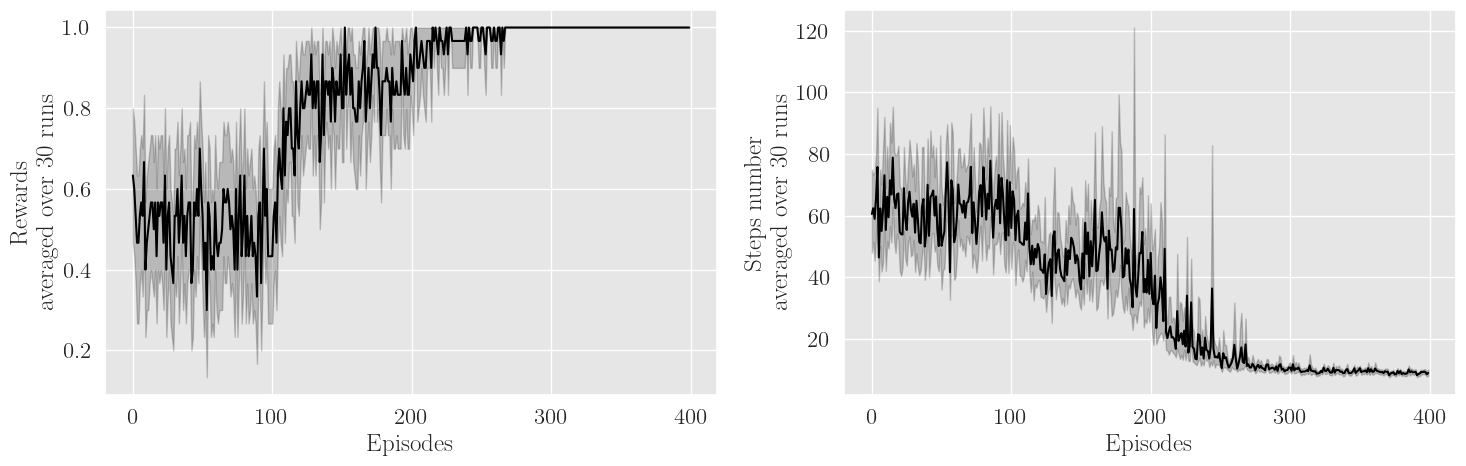
\includegraphics[width=0.85\textwidth]{medias/LeftRight/training.png}
\end{center}

East/West
\begin{center}
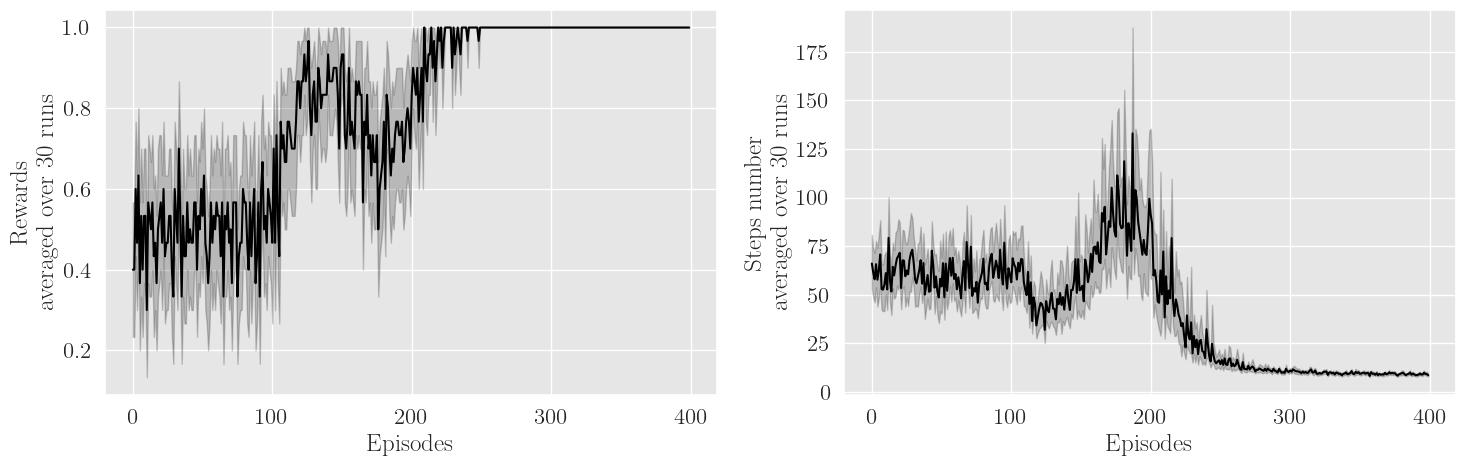
\includegraphics[width=0.85\textwidth]{medias/EastWest/training.png}
\end{center}
\end{frame}
\begin{frame}[label={sec:orgd9631a1}]{Randomized Cartesian inputs}
\centering
Left/Right
\begin{center}
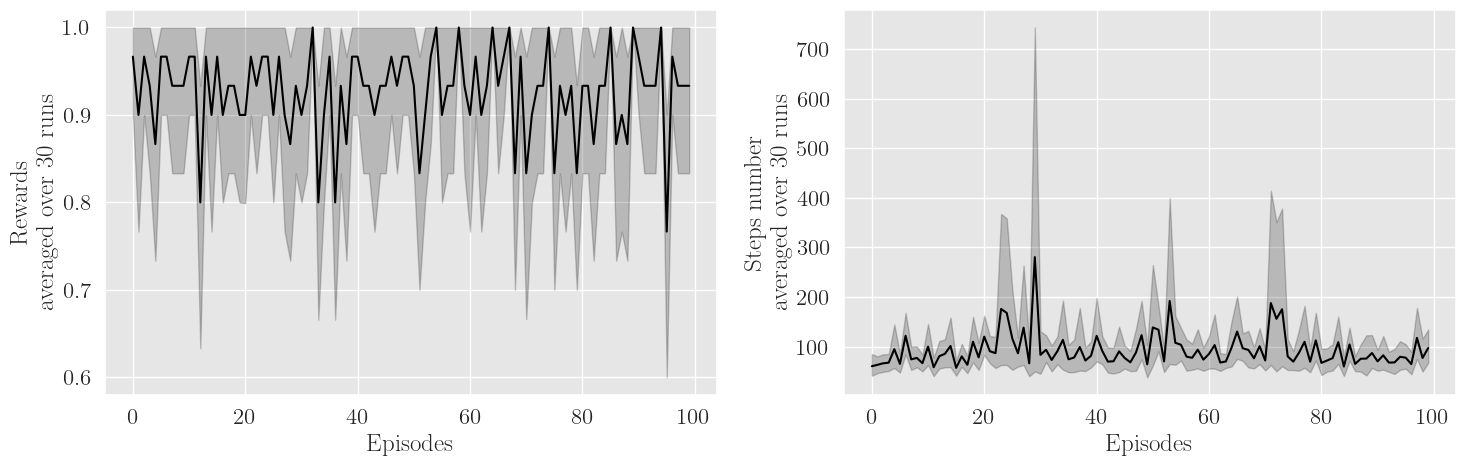
\includegraphics[width=0.85\textwidth]{medias/LeftRight/exp_keep-polar_silence-False.png}
\end{center}

East/West
\begin{center}
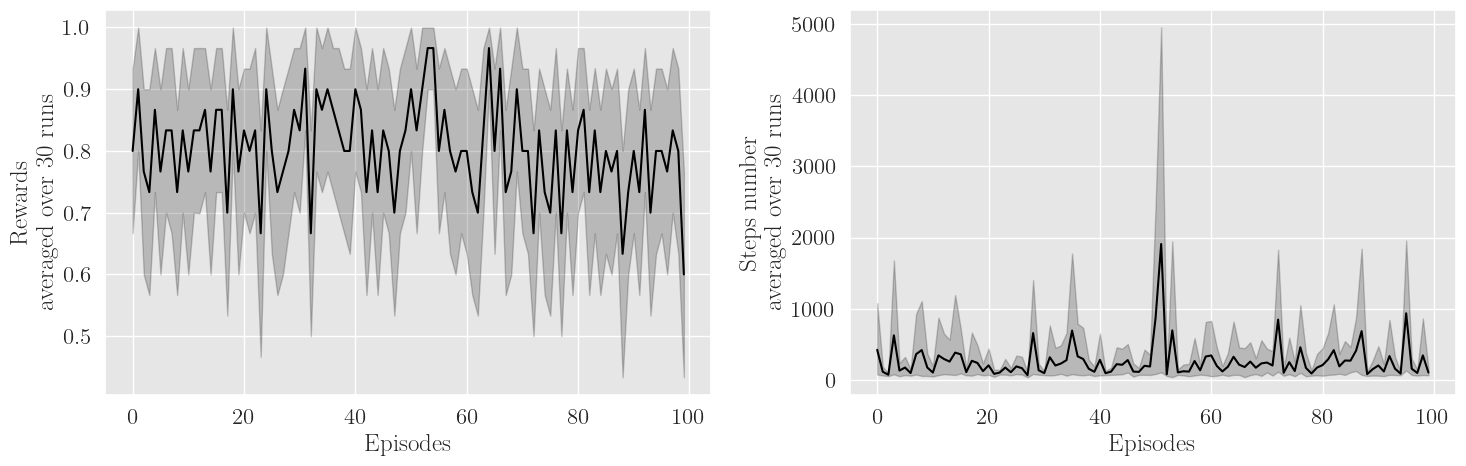
\includegraphics[width=0.85\textwidth]{medias/EastWest/exp_keep-polar_silence-False.png}
\end{center}
\end{frame}
\begin{frame}[label={sec:org7a6918c}]{Silenced Cartesian inputs}
\centering
Left/Right
\begin{center}
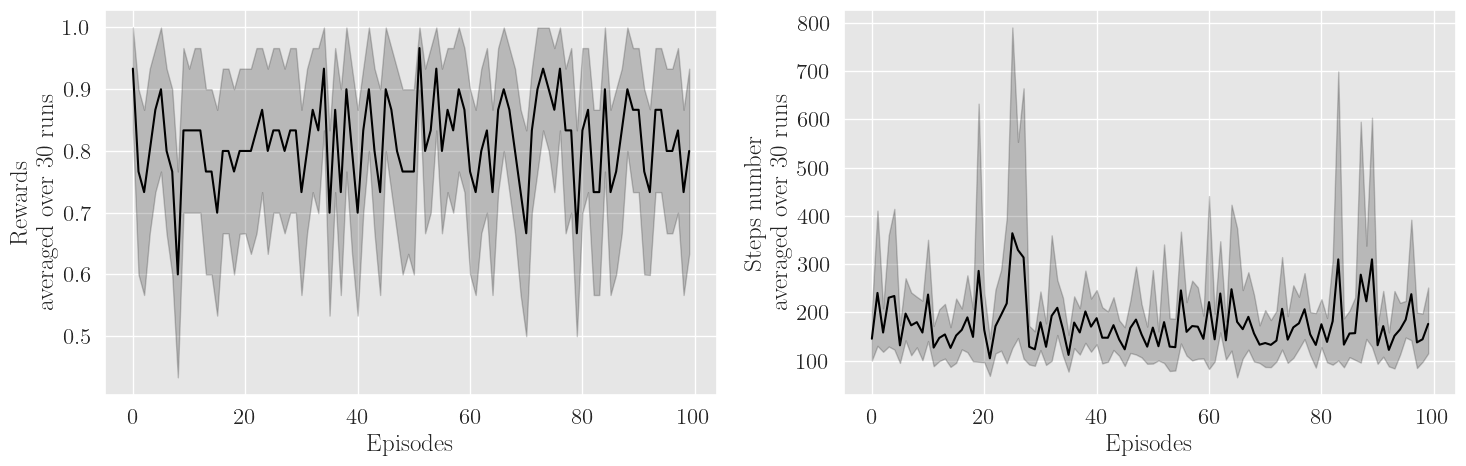
\includegraphics[width=0.85\textwidth]{medias/LeftRight/exp_keep-polar_silence-True.png}
\end{center}

East/West
\begin{center}
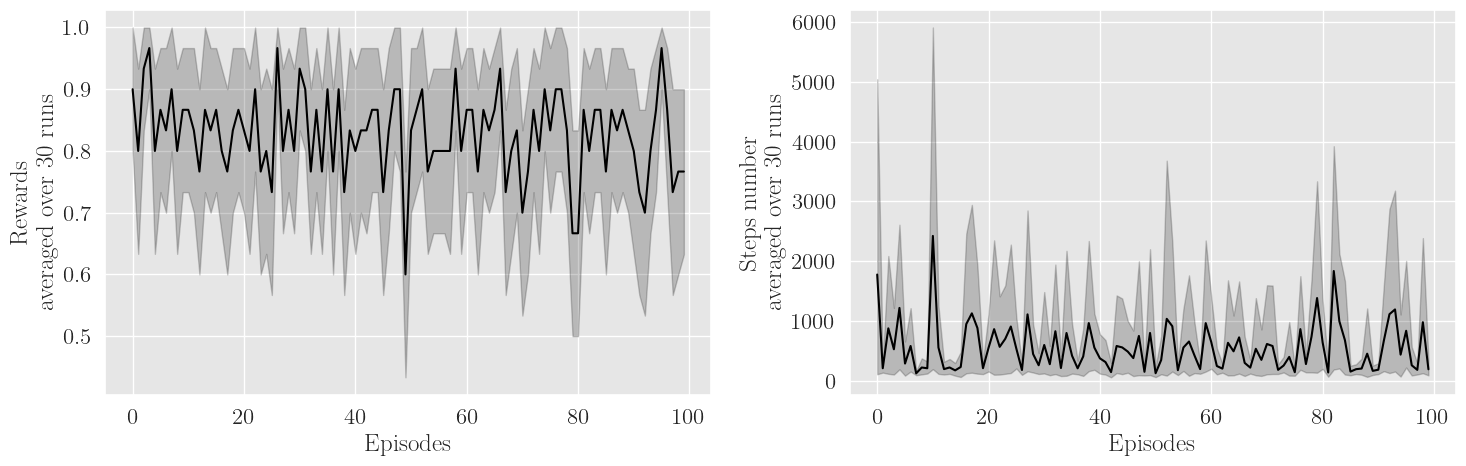
\includegraphics[width=0.85\textwidth]{medias/EastWest/exp_keep-polar_silence-True.png}
\end{center}
\end{frame}
\begin{frame}[label={sec:org9d78291}]{Randomized polar inputs}
\centering
Left/Right
\begin{center}
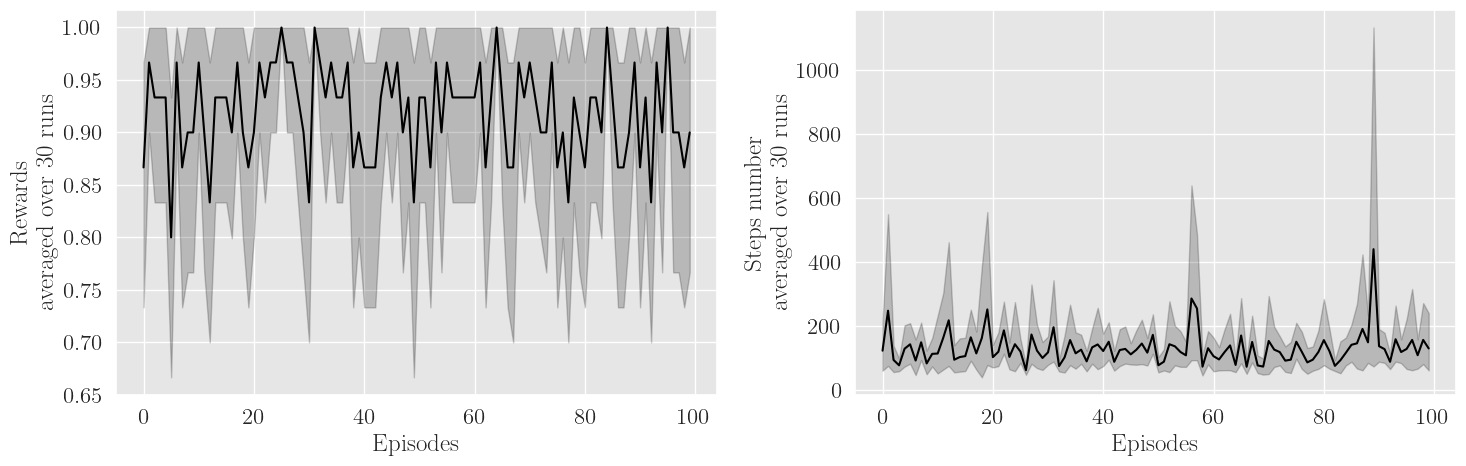
\includegraphics[width=0.85\textwidth]{medias/LeftRight/exp_keep-cartesian_silence-False.png}
\end{center}

East/West
\begin{center}
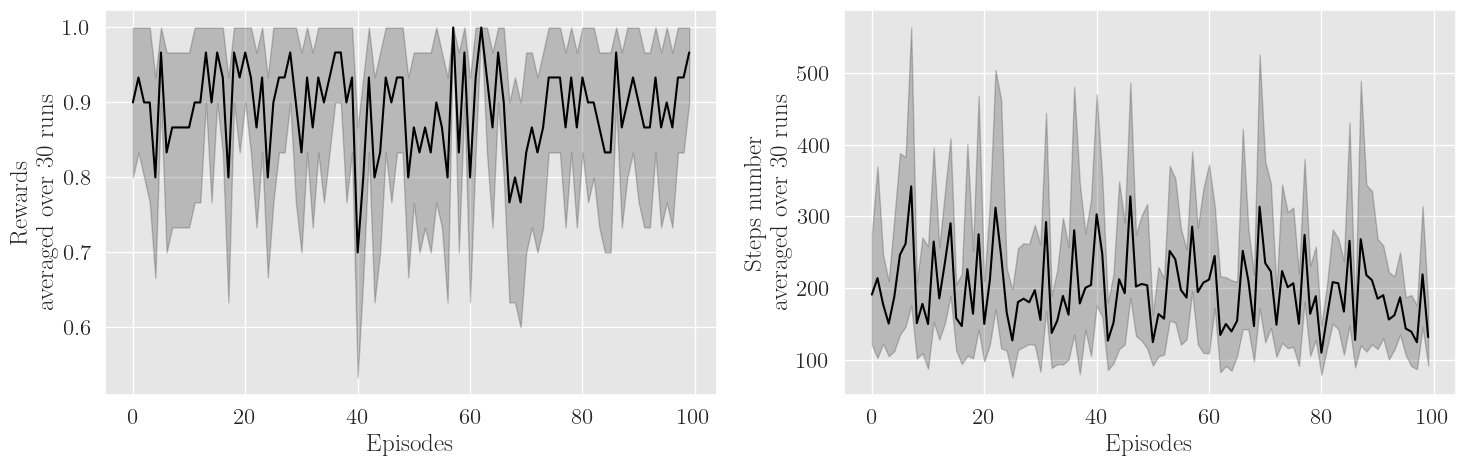
\includegraphics[width=0.85\textwidth]{medias/EastWest/exp_keep-cartesian_silence-False.png}
\end{center}
\end{frame}
\begin{frame}[label={sec:org0903287}]{Silenced polar inputs}
\centering
Left/Right
\begin{center}
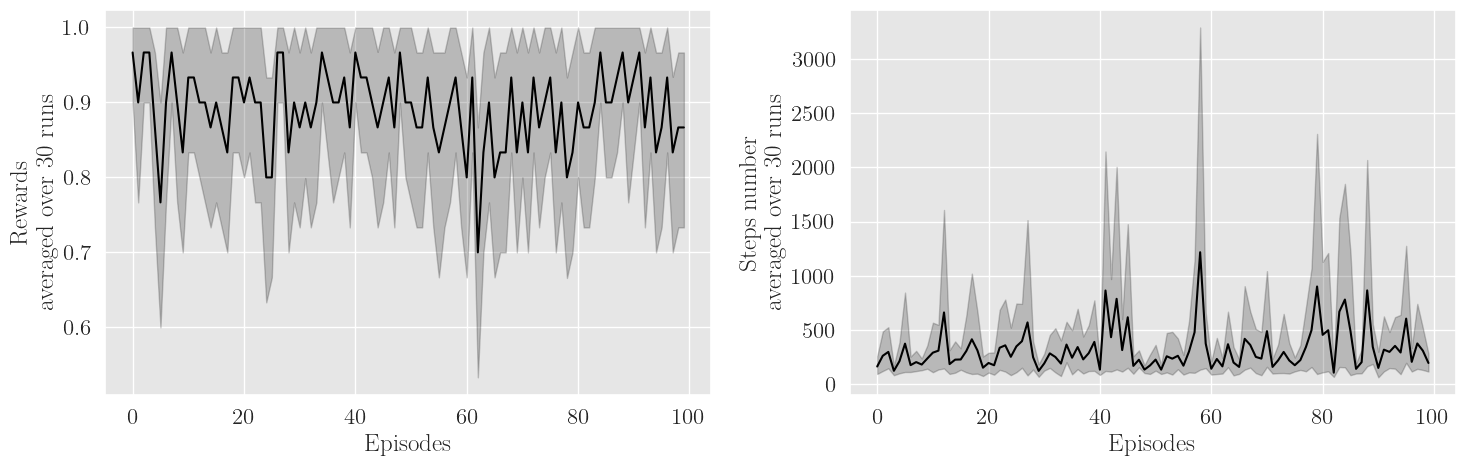
\includegraphics[width=0.85\textwidth]{medias/LeftRight/exp_keep-cartesian_silence-True.png}
\end{center}

East/West
\begin{center}
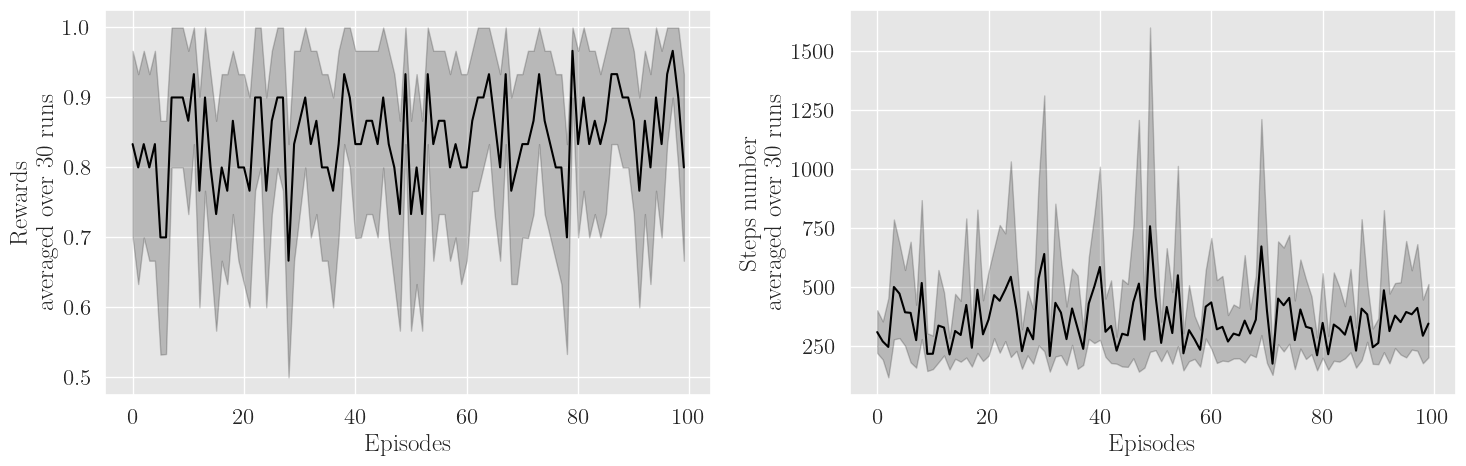
\includegraphics[width=0.85\textwidth]{medias/EastWest/exp_keep-cartesian_silence-True.png}
\end{center}
\end{frame}
\section{Conclusion}
\label{sec:org1cca607}
\begin{frame}[label={sec:org326229a}]{Conclusion}
\begin{itemize}
\item Results not as expected \(\to\) performance is degraded but the agents are able to solve the task most of the time even if part of their inputs are perturbated
\item Changes from lab meeting:
\begin{itemize}
\item One-hot encoded cue
\item 256 neurons/layer instead of 512
\end{itemize}
\end{itemize}
\end{frame}
\end{document}
